\documentclass[11pt,a4paper]{article}
\usepackage[margin=2.3cm]{geometry}
\usepackage[T1]{fontenc}
\usepackage{textcomp}
\input{glyphtounicode}
\pdfgentounicode=1
\usepackage{lmodern}
\usepackage{amsmath}
\usepackage{xcolor}
\usepackage{listings}
\usepackage{tcolorbox}
\usepackage{booktabs}
\usepackage{array}
\usepackage{tikz}
\usepackage{hyperref}
\hypersetup{colorlinks=true, linkcolor=blue!50!black, citecolor=green!40!black}

\definecolor{codebg}{RGB}{248,248,245}
\lstset{
  language=C, basicstyle=\ttfamily\footnotesize, backgroundcolor=\color{codebg},
  keywordstyle=\color{blue!60!black}\bfseries, commentstyle=\color{green!45!black}\itshape,
  stringstyle=\color{red!60!black}, numbers=none, upquote=true,
  frame=single, rulecolor=\color{gray!40}, breaklines=true, columns=fullflexible,
  keepspaces=true, showstringspaces=false
}
\lstdefinestyle{sh}{language=bash, backgroundcolor=\color{black!5}}

\newtcolorbox{keyidea}{colback=blue!4, colframe=blue!45!black, title=Key ideas, fonttitle=\bfseries\small}
\newtcolorbox{experiment}{colback=orange!5, colframe=orange!70!black, title=Experiment, fonttitle=\bfseries\small}

\title{\textbf{OpenMP --- Lesson 5}\\[4pt]\large Load balancing: the \texttt{schedule} clause}
\author{Gustavo Lozano}
\date{November 2026}

\begin{document}
\maketitle

\noindent\textit{\small Sources: Chapman, Jost \& van der Pas~\cite{chapman}, Ch.~4
``OpenMP Language Features'' (the \texttt{schedule} and \texttt{nowait} clauses) and
Ch.~5 ``How to Get Good Performance'' (load imbalance).}

\section{The idea}
In Lesson~4 every iteration cost the same, so cutting the loop into $p$ equal blocks was
perfect. Now suppose iteration $i$ costs work proportional to $i$. With two threads and
equal blocks, thread~0 gets iterations $0,\dots,499$ and thread~1 gets
$500,\dots,999$. Thread~1 has about \textbf{three times} more work:
\[
  \sum_{i=0}^{499} i \approx \tfrac14 \sum_{i=0}^{999} i,
  \qquad
  \sum_{i=500}^{999} i \approx \tfrac34 \sum_{i=0}^{999} i .
\]
Thread~0 finishes early and sits idle at the barrier, while thread~1 is still working.
The loop takes as long as the \emph{slowest} thread. This is \textbf{load imbalance}.

\begin{center}
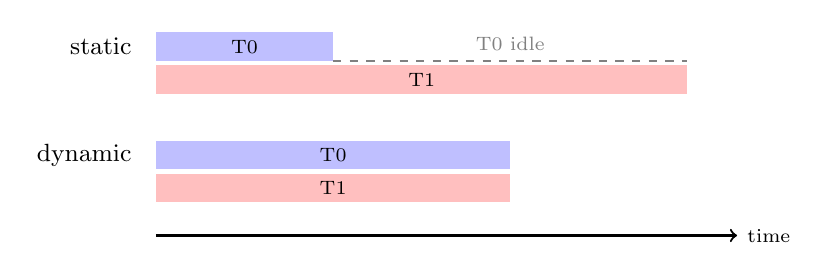
\begin{tikzpicture}[thick, x=0.9cm, y=0.6cm]
  \node[font=\small, anchor=east] at (-0.2,1) {static};
  \fill[blue!25] (0,0.7) rectangle (2.5,1.3);   \node[font=\scriptsize] at (1.25,1) {T0};
  \fill[red!25]  (0,0.0) rectangle (7.5,0.6);   \node[font=\scriptsize] at (3.75,0.3) {T1};
  \draw[dashed, gray] (2.5,0.7) -- (7.5,0.7) node[midway, above, font=\scriptsize] {T0 idle};
  \node[font=\small, anchor=east] at (-0.2,-1.3) {dynamic};
  \fill[blue!25] (0,-1.0) rectangle (5,-1.6);   \node[font=\scriptsize] at (2.5,-1.3) {T0};
  \fill[red!25]  (0,-1.7) rectangle (5,-2.3);   \node[font=\scriptsize] at (2.5,-2.0) {T1};
  \draw[->] (0,-3) -- (8.2,-3) node[right, font=\scriptsize] {time};
\end{tikzpicture}
\end{center}

\section{The \texttt{schedule} clause}
\texttt{schedule(kind[, chunk])} on an \texttt{omp for} decides which thread gets which
iterations.
\begin{center}
\small
\begin{tabular}{@{}>{\raggedright\arraybackslash}p{3.0cm}>{\raggedright\arraybackslash}p{8.2cm}>{\raggedright\arraybackslash}p{4.0cm}@{}}
\toprule
Kind & How iterations are assigned & Good for \\ \midrule
\texttt{static} & split into $p$ contiguous blocks \emph{before} the loop starts
  (with \texttt{chunk}: blocks of size \texttt{chunk} dealt round-robin) & equal-cost iterations; lowest overhead \\
\texttt{dynamic, chunk} & a thread takes \texttt{chunk} iterations; when done, it asks for the
  next free chunk (default chunk = 1) & unequal or unpredictable cost \\
\texttt{guided} & like \texttt{dynamic}, but chunks start large and shrink as the loop
  progresses & unequal cost, fewer requests \\
\bottomrule
\end{tabular}
\end{center}

\paragraph{The \texttt{nowait} clause.} The \texttt{omp for} loop normally ends with an
implicit barrier. \texttt{nowait} removes it, so a thread that finishes its share continues
immediately. Here we use it only to \emph{measure} when each thread finishes; the end of the
\texttt{parallel} region still has its own barrier.

\section{The code}
The program runs the same unequal loop three times, once per schedule, and prints when
each thread finished and the total time.
\lstinputlisting[title=\texttt{schedule.c}]{schedule.c}

\begin{lstlisting}[style=sh]
gcc -Wall -fopenmp -o schedule schedule.c
OMP_NUM_THREADS=2 ./schedule
\end{lstlisting}
Typical output on 2 cores (your times will differ):
\begin{lstlisting}[style=sh]
static             total 0.156 s   finish per thread: 0.063 0.155
dynamic,1          total 0.102 s   finish per thread: 0.102 0.102
guided             total 0.105 s   finish per thread: 0.105 0.105
\end{lstlisting}

\begin{keyidea}
\begin{itemize}
  \item With \texttt{static}, thread 0 finishes at about $1/3$ of the time of thread 1:
        exactly the $1/4$ vs.\ $3/4$ split of the work computed above.
  \item With \texttt{dynamic} and \texttt{guided}, all threads finish together. Nobody is
        idle, so the total time drops.
  \item The schedule does not change the \emph{result}, only \emph{who} does
        \emph{which} iteration and therefore the time.
  \item \texttt{static} is decided once, at no cost. \texttt{dynamic} pays a small cost
        every time a thread asks for a new chunk. Use it when the cost of iterations
        varies.
\end{itemize}
\end{keyidea}

\section{The experiment}
\begin{experiment}
\textbf{Question:} which schedule balances unequal work, and what does balancing cost?
\begin{enumerate}
  \item Run with 1 thread and with $p =$ \texttt{nproc} threads:
\begin{lstlisting}[style=sh]
OMP_NUM_THREADS=1 ./schedule
OMP_NUM_THREADS=$(nproc) ./schedule
\end{lstlisting}
  \item For $p =$ \texttt{nproc}, compare the per-thread finish times of each schedule.
  \item Compare the three totals in the 1-thread run.
\end{enumerate}
\textbf{What to observe and answer.}
\begin{enumerate}
  \item With \texttt{static}, which thread finishes last? Predict the ratio between the
        first and last finish time from the work formula, and check it.
  \item Why do \texttt{dynamic} and \texttt{guided} make all threads finish at the same time?
  \item With 1 thread there is nothing to balance, yet \texttt{dynamic} and
        \texttt{guided} are a bit slower than \texttt{static}. Why?
\end{enumerate}
\end{experiment}

\paragraph{Answers (read after trying).}
(1)~The last thread, because it owns the most expensive iterations. With $p$ threads,
block $k$ holds a share of the work proportional to $2k+1$, so with 2 threads the ratio is
$1:3$, and with 4 threads $1:3:5:7$.
(2)~Work is handed out on demand. A thread that drew cheap iterations comes back sooner and
takes more of them, so all threads stay busy until the loop runs out.
(3)~Scheduling overhead. \texttt{dynamic,1} makes one request per iteration (1000
requests) even when there is no other thread to share with. \texttt{static} decides
everything once, before the loop. The general rule: use \texttt{static} when iterations cost
the same, \texttt{dynamic} or \texttt{guided} when they do not.

\paragraph{Next lesson.} Beyond loops: the \texttt{sections} and \texttt{single}
constructs, and the explicit \texttt{barrier} (Chapman et al., Ch.~4).

\begin{thebibliography}{9}
\bibitem{chapman} B.~Chapman, G.~Jost, and R.~van der Pas. \emph{Using OpenMP: Portable
  Shared Memory Parallel Programming}. MIT Press, Cambridge, MA, 2007.
\end{thebibliography}
\end{document}
